\section{Proposition de l'article}

L'article étudié se propose de réunir les deux algorithmes précédents (ICP et Point-to-plane ICP) dans un cadre probabiliste commun. Ce cadre commun permet d'autre part de développer une nouvelle variante de l'algorithme dénommée "Plane-to-plane" ICP.\\

Le framework probabiliste décrit dans \cite{bib_gicp} ne concerne que l'énergie utilisée pour trouver la transformation optimale. En effet, l'étape de recherche de plus proche voisin n'a pas été modifiée afin de conserver la rapidité de recherche des plus proche voisins (En utilisant des kd-tree, la recherche se fait en complexité $\mathcal{O}(n\log{}n)$).\\

La composante probabiliste de GICP est donc introduite dans l'étape de minimisation de l'énergie. Au lieu de considérer les nuages de points $A = \{a_{i}\}_{i=1..N}$ et $B = \{b_{i}\}_{i=1..N}$ comme étant des nuages de points déterministes, on considère $A$ et $B$ comme étant une réalisation d'un processus aléatoire généré à partir de  $\hat{A} = \{\hat{a}_{i}\}_{i=1..N}$ et $\hat{B} = \{\hat{b}_{i}\}_{i=1..N}$ pour lequel $a_{i} \sim \mathcal{N}(\hat{a_{i}}, C_{i}^A)$ et $b_{i} \sim \mathcal{N}(\hat{b_{i}}, C_{i}^B)$. Cela correspond à dire qu'il y a une forte probabilité pour que le point $a_{i}$ se trouve en $\hat{a}_i$, mais qu'il n'est pas impossible qu'il soit un peu déplacé dans le voisinage de $\hat{a_{i}}$.\\

Dans ce cadre, si on connait la transformation optimale $\mathbf{T}^{*}$, on a $\hat{b_{i}} = \mathbf{T}^{*}\hat{a}_{i}$. On peut définir $d_{i}^{T} = b_{i} - \mathbf{T}a_{i}$ pour une transformation rigide $\mathbf{T}$. Comme $a_{i}$ et $b_{i}$ suivent des distributions gaussiennes indépendantes, on a :
\begin{eqnarray}
d_{i}^{(\mathbf{T}^{*})} &\sim& \mathcal{N}(\hat{b_{i}}-(\mathbf{T}^{*})a_{i},C_{i}^B + (\mathbf{T}^{*})C_{i}^{A}(\mathbf{T}^{*T}))\\
&=& \mathcal{N}(0,C_{i}^B + (\mathbf{T}^{*})C_{i}^{A}(\mathbf{T}^{*})^{T})
\end{eqnarray}

On souhaite minimiser la distance $d_{i}^{\mathbf{T}}$, ainsi on souhaite maximiser la probabilité que $d_{i}^{\mathbf{T}}$ soit égal à 0. On utilise l'estimation du maximum de vraisemblance afin d'estimer les paramètres de la transformation $\mathbf{T}$.

\begin{eqnarray}
\mathbf{T} &=& \underset{\mathbf{T}}{\text{arg max}} \prod_{i} p(d_{i}^{(\mathbf{T})}) \\
&=& \underset{\mathbf{T}}{\text{arg max}} \sum_{i} log(p(d_{i}^{(\mathbf{T})})) \\
&=& \underset{\mathbf{T}}{\text{arg min}} \sum_{i} d_{i}^{(\mathbf{T})^T}(C_{i}^B + \mathbf{T}^{T}C_{i}^{A}\mathbf{T})^{-1}d_{i}^{(\mathbf{T})}
\end{eqnarray}

Le terme d'erreur unitaire $d_{i}^{(\mathbf{T})^T}(C_{i}^B+\mathbf{T}^{T}C_{i}^{A}\mathbf{T})^{-1}d_{i}^{(\mathbf{T})}$  est une distance probabiliste qui prends en compte la densité de probabilité des points dans l'espace $\mathbb{R}^{3})$. Jusqu'à maintenant, les matrice de covariance $C_{i}^A$ et $C_{i}^B$ n'ont pas été définie. C'est le choix de ces matrices qui va déterminer dans quel cadre on souhaite résoundre la minimisation.\\

En effet, si l'on choisi $C_{i}^B = Id$ et $C_{i}^A = 0$, on se place par exemple dans le cadre de l'ICP standard :

\begin{eqnarray}
\mathbf{T} &=& \underset{\mathbf{T}}{\text{arg min}} \sum_{i} d_{i}^{(\mathbf{T})^T}(C_{i}^B + \mathbf{T}^{T}C_{i}^{A}\mathbf{T})^{-1}d_{i}^{(\mathbf{T})}\\
&=& \underset{\mathbf{T}}{\text{arg min}} \sum_{i} d_{i}^{(\mathbf{T})^T}(Id)^{-1}d_{i}^{(\mathbf{T})}\\
&=& \underset{\mathbf{T}}{\text{arg min}} \sum_{i} \|d_{i}^{(\mathbf{T})}\|^2\\
\end{eqnarray}

Dans \cite{bib_gicp}, Segal et al. proposent une extension de l'ICP standard et du Point-to-plane ICP  dénommée Plane-to-plane. Pour faire cette extension, il est posé comme hypothèse que les nuages de points sont localement plans. D'autre part, comme les scans ne sont pas pris du même point de vue, il est très fortement probable que les correspondances ne sont pas exactes. Cependant, des points proches seront tout de même situés sur le même plan. Pour modéliser ce phénomène, la matrice de covariance est construite pour avoir un très faible coefficient le long de la normale. Plus précisément, si la normale est colinéaire à $e1$, la matrice de covariance s'écrit sous la forme 

\begin{equation}C_{plan} = \begin{pmatrix} 
 \epsilon & 0 & 0 \\
 0 & 1 & 0 \\ 
 0 & 0 & 1 
 \end{pmatrix}
\end{equation}

Afin de calculer ces matrices de covariances dans le cas de nuages de points réel, il y a donc une étape d'estimation des normales du nuage de point. Les auteurs indiquent utiliser une méthode d'estimation de normales par PCA sur les 20 plus proches voisins. En pratique, cela consiste à trouver dans le nuage de points les 20 plus proches voisins du point où l'on cherche à estimer la normale. Dans un second temps, on calcule la matrice de covariance $\hat{\Sigma}$ de l'ensemble de ces points. Enfin, on calcule la SVD de $\hat{\Sigma}$ : $\hat{\Sigma} = UDU^{T}$. La matrice $U$ contient les vecteurs propres de la matrice de covariance des points, et le vecteur qui correspond à la plus petite valeur propre est dans la direction de la normale. Ainsi, en remplaçant la matrice D par la matrice décrite plus haut on a (dans le cas ou la plus petite valeur propre correspond au premier vecteur propre) :

\begin{equation}
C_{i}^B = U_{i}^B.\begin{pmatrix} 
 \epsilon & 0 & 0 \\
 0 & 1 & 0 \\ 
 0 & 0 & 1 
 \end{pmatrix}.{U_{i}^{B}}^T
\end{equation}

On peut réaliser le même calcul pour $C_{i}^A$.

L'intuition de l'influence de ces matrices de covariance est la suivante :\\

\begin{itemize}
\item{Dans le cas ou les normales sont colinéaires après transformation du second nuage de point, la somme des matrices de covariances $C_{i}^B + \mathbf{T}^{T}C_{i}^{A}\mathbf{T}$ est une matrice qui reste anisotrope. La distance unitaire ${d_{i}^{\mathbf{T}}}^{T}(C_{i}^B + \mathbf{T}^{T}C_{i}^{A}\mathbf{T})d_{i}^{\mathbf{T}}$ sera donc fortement impactée si les points sont éloignés dans la direction de la normale.  
}

\item{Dans le cas ou les normales ne sont pas colinéaires (par exemple dans le cas extrêmes ou elles sont orthogonales}, la somme des matrices de covariances va être de plus en plus isotrope. Ainsi la distance unitaire calculée ${d_{i}^{\mathbf{T}}}^{T}(C_{i}^B + \mathbf{T}^{T}C_{i}^{A}\mathbf{T})d_{i}^{\mathbf{T}}$ aura moins d'influence dans le calcul de la fonction de coût.
\end{itemize}

L'image \ref{fig_cov} représente deux points pour lesquels les normales sont colinéaires, et deux points pour lesquelles les normales sont orthogonales, et l'influence que ces normales ont sur le calcul de la distance unitaire entre ces deux points.

\begin{figure}[H]
\centering
\begin{tabular}{cc}
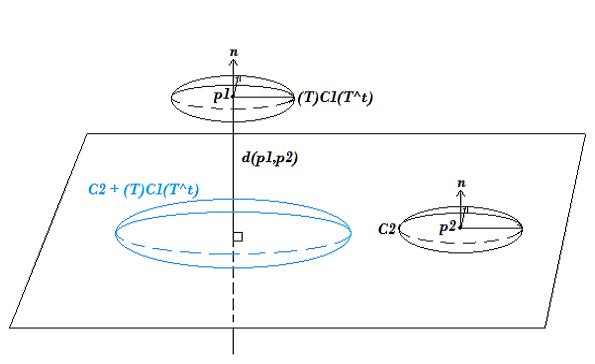
\includegraphics[width = 0.5\textwidth]{Images/Proposition/covcol} &
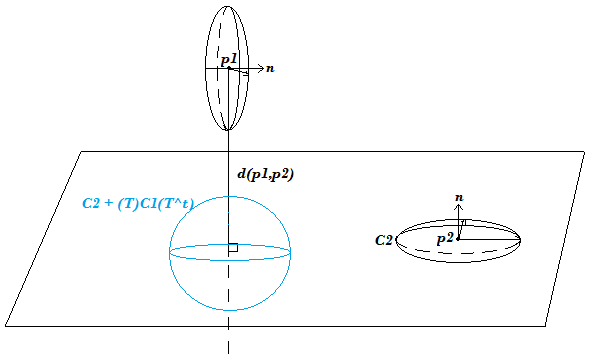
\includegraphics[width = 0.5\textwidth]{Images/Proposition/covorth}
\end{tabular}
\caption{Influence des matrices de covariance sur le calcul de distance}
\label{fig_cov}
\end{figure}






